\uuid{3hQ7}
\titre{Série de Fourier de la fonction $x\mapsto |\sin (x/2)|$ }

\niveau{L2}
\module{Séries de Fourier}
\chapitre{Séries de Fourier}
\sousChapitre{Dirichlet et Parseval}
\theme{Fonction périodique paire}
\auteur{Quentin Liard}
\datecreate{ 2026-04-10}
\organisation{AMSCC}
\difficulte{4}

\contenu{

\texte{ 
On considère la fonction $f$ définie sur $\mathbb{R}$ par
$$
f(x)=|\sin (x/2)|.
$$

}

\begin{enumerate}
\item \question{Représenter la fonction $f$ sur l'intervalle $[-2\pi;2\pi]$.}
\reponse{
\begin{center}
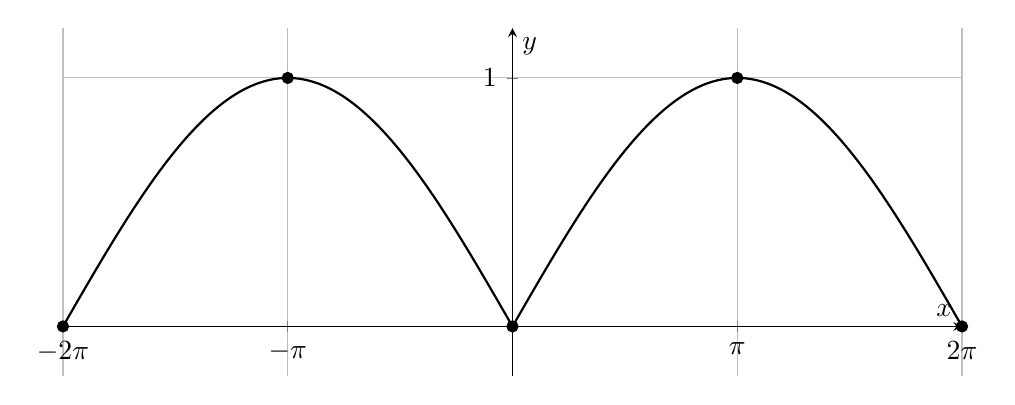
\begin{tikzpicture}
\begin{axis}[
    axis lines=middle,
    xmin=-2*pi, xmax=2*pi,
    ymin=-0.2, ymax=1.2,
    samples=300,
    domain=-2*pi:2*pi,
    xtick={-2*pi,-pi,0,pi,2*pi},
    xticklabels={$-2\pi$,$-\pi$,$0$,$\pi$,$2\pi$},
    ytick={0,1},
    xlabel={$x$},
    ylabel={$y$},
    width=13cm,
    height=6cm,
    grid=both
]
\addplot[thick] {abs(sin(deg(x/2)))};

\addplot[only marks, mark=*, mark size=2pt] coordinates {
    (-2*pi,0) (-pi,1) (0,0) (pi,1) (2*pi,0)
};
\end{axis}
\end{tikzpicture}
\end{center}


Sur $[0,2\pi]$, on a $\sin(x/2)\ge 0$, donc
$$
f(x)=\sin(x/2).
$$
Sur $[-2\pi,0]$, on a $\sin(x/2)\le 0$, donc
$$
f(x)=-\sin(x/2).
$$
Ainsi, sur l’intervalle $[-2\pi,2\pi]$, la courbe est formée de deux arches positives :
\begin{itemize}
\item $f(-2\pi)=0$, $f(-\pi)=1$, $f(0)=0$ ;
\item $f(0)=0$, $f(\pi)=1$, $f(2\pi)=0$.
\end{itemize}
La fonction est donc positive, nulle en $-2\pi$, $0$ et $2\pi$, et atteint son maximum $1$ en $-\pi$ et en $\pi$.
}

\item \question{Montrer que, pour tout $x$ réel et pour tout $n\geq 1$:
$$
\sin (x/2)\cos(nx)=\frac12\left(\sin \left((n+\frac 12)x\right)-\sin \left((n-\frac 12)x\right)\right).
$$
On pourra admettre cette formule dans la suite.}
\reponse{
On utilise la formule trigonométrique classique
$$
\sin a\cos b=\frac12\bigl(\sin(a+b)+\sin(a-b)\bigr).
$$
En prenant
$$
a=\frac{x}{2}
\qquad\text{et}\qquad
b=nx,
$$
on obtient
$$
\sin(x/2)\cos(nx)
=
\frac12\left(\sin\left(\left(n+\frac12\right)x\right)+\sin\left(\left(\frac12-n\right)x\right)\right).
$$
Or
$$
\sin\left(\left(\frac12-n\right)x\right)=-\sin\left(\left(n-\frac12\right)x\right).
$$
Donc
$$
\sin (x/2)\cos(nx)=\frac12\left(\sin \left((n+\frac 12)x\right)-\sin \left((n-\frac 12)x\right)\right).
$$
}

\item \question{Montrer que la fonction $f$ est $2\pi-$périodique et paire.}
\reponse{
Pour tout $x\in\mathbb{R}$,
$$
f(x+2\pi)=\left|\sin\left(\frac{x+2\pi}{2}\right)\right|
=\left|\sin\left(\frac{x}{2}+\pi\right)\right|
=\left|-\sin\left(\frac{x}{2}\right)\right|
=\left|\sin\left(\frac{x}{2}\right)\right|
=f(x).
$$
Donc $f$ est $2\pi$-périodique.

De plus, pour tout $x\in\mathbb{R}$,
$$
f(-x)=\left|\sin\left(-\frac{x}{2}\right)\right|
=\left|-\sin\left(\frac{x}{2}\right)\right|
=\left|\sin\left(\frac{x}{2}\right)\right|
=f(x).
$$
Ainsi, $f$ est paire.
}

\item   \question{Calculer les coefficients de Fourier de $f$ et écrire $S(f)$ la série de Fourier de $f$.}
\indication{}
\reponse{
Comme $f$ est paire et $2\pi$-périodique, sa série de Fourier ne contient que des cosinus :
$$
S(f)(x)=\frac{a_0}{2}+\sum_{n\ge 1} a_n\cos(nx),
$$
avec
$$
a_0=\frac{1}{\pi}\int_{-\pi}^{\pi}f(x)\,dx,
\qquad
a_n=\frac{1}{\pi}\int_{-\pi}^{\pi}f(x)\cos(nx)\,dx,
\qquad
b_n=0.
$$

Sur $[0,\pi]$, on a $f(x)=\sin(x/2)$, donc
$$
a_0=\frac{2}{\pi}\int_0^\pi \sin(x/2)\,dx.
$$
Or
$$
\int \sin(x/2)\,dx=-2\cos(x/2),
$$
donc
$$
a_0=\frac{2}{\pi}\left[-2\cos(x/2)\right]_0^\pi
=\frac{2}{\pi}(2)=\frac{4}{\pi}.
$$
Ainsi
$$
\frac{a_0}{2}=\frac{2}{\pi}.
$$

Pour $n\ge 1$,
$$
a_n=\frac{2}{\pi}\int_0^\pi \sin(x/2)\cos(nx)\,dx.
$$
En utilisant la formule admise à la question précédente,
$$
\sin(x/2)\cos(nx)
=
\frac12\left(\sin\left(\left(n+\frac12\right)x\right)-\sin\left(\left(n-\frac12\right)x\right)\right),
$$
d’où
$$
a_n=\frac{1}{\pi}\int_0^\pi
\left(\sin\left(\left(n+\frac12\right)x\right)-\sin\left(\left(n-\frac12\right)x\right)\right)\,dx.
$$
Or, pour tout réel $\lambda\neq 0$,
$$
\int_0^\pi \sin(\lambda x)\,dx
=
\left[-\frac{\cos(\lambda x)}{\lambda}\right]_0^\pi
=
\frac{1-\cos(\lambda\pi)}{\lambda}.
$$
Ici,
$$
\cos\left(\left(n+\frac12\right)\pi\right)=0
\qquad\text{et}\qquad
\cos\left(\left(n-\frac12\right)\pi\right)=0.
$$
Donc
$$
\int_0^\pi \sin\left(\left(n+\frac12\right)x\right)\,dx
=
\frac{1}{n+\frac12},
$$
et
$$
\int_0^\pi \sin\left(\left(n-\frac12\right)x\right)\,dx
=
\frac{1}{n-\frac12}.
$$
Ainsi
$$
a_n
=
\frac{1}{\pi}\left(\frac{1}{n+\frac12}-\frac{1}{n-\frac12}\right).
$$
On simplifie :
$$
\frac{1}{n+\frac12}-\frac{1}{n-\frac12}
=
\frac{n-\frac12-(n+\frac12)}{\left(n+\frac12\right)\left(n-\frac12\right)}
=
\frac{-1}{n^2-\frac14}
=
-\frac{4}{4n^2-1}.
$$
Donc
$$
a_n=-\frac{4}{\pi(4n^2-1)}.
$$

Finalement,
$$
b_n=0,
\qquad
a_0=\frac{4}{\pi},
\qquad
a_n=-\frac{4}{\pi(4n^2-1)}\quad (n\ge 1).
$$
La série de Fourier de $f$ est donc
$$
\boxed{
S(f)(x)=\frac{2}{\pi}-\frac{4}{\pi}\sum_{n\ge 1}\frac{\cos(nx)}{4n^2-1}.
}
$$

%Comme $f$ est continue et $2\pi$-périodique, le théorème de Dirichlet assure que cette série converge vers $f(x)$ pour tout $x\in\mathbb{R}$.
}

\end{enumerate}

}